\documentclass{beamer}
\usepackage{tikz}
\usetikzlibrary{arrows.meta, decorations.pathreplacing, calc}

% ------------------------------------------------------------------
% Theme colors & styles: blkline / blkfill / accentline / accentfill /
% lbl / flow. Assumed to already exist in your master preamble — delete
% this block if dropping this frame into that file.
% ------------------------------------------------------------------
\definecolor{blkline}{HTML}{375775}
\definecolor{blkfill}{HTML}{EAF0F7}
\definecolor{accentline}{HTML}{B5651D}
\definecolor{accentfill}{HTML}{FBEEDD}
\tikzset{
  lbl/.style={text=black},
  flow/.style={-{Stealth[length=2.2mm]}, thick},
  loadedbox/.style={draw=blkline, fill=blkfill, thick},          % register: known value
  extbox/.style={draw=blkline, fill=blkfill!35, thick, dashed},  % register: garbage/undefined
  memwrite/.style={draw=accentline, fill=accentfill, thick},          % memory: known value
  memkeep/.style={draw=accentline, fill=accentfill!35, thick, dashed}, % memory: garbage/undefined
}

\begin{document}

\begin{frame}{Data Copy: LDR / LDR / LDR / STR}

\begin{center}
\begin{tabular}{l}
\alt<2>{\textcolor{accentline}{\bfseries\ttfamily ldr r0, =0x2000}}{\ttfamily ldr r0, =0x2000}\\[2pt]
\alt<3>{\textcolor{accentline}{\bfseries\ttfamily ldr r1, =0x2004}}{\ttfamily ldr r1, =0x2004}\\[2pt]
\alt<4>{\textcolor{accentline}{\bfseries\ttfamily ldr r2, [r0]}}{\ttfamily ldr r2, [r0]}\\[2pt]
\alt<5>{\textcolor{accentline}{\bfseries\ttfamily str r2, [r1]}}{\ttfamily str r2, [r1]}
\end{tabular}
\end{center}

\vspace{1mm}
{\small\itshape
\only<1>{Initial state: R0, R1, R2 hold garbage; [0x2000] already holds the data to copy.}%
\only<2>{Step 1: R0 is loaded with the source address 0x2000.}%
\only<3>{Step 2: R1 is loaded with the destination address 0x2004.}%
\only<4>{Step 3: the word at address [R0] is read from memory into R2.}%
\only<5>{Step 4: R2 is written back out to memory at address [R1] — the copy is complete.}%
\par}

\vspace{2mm}
\resizebox{0.95\textwidth}{!}{%
\begin{tikzpicture}[x=10mm, y=8mm]

% Fix the bounding box so resizebox scales identically on every overlay.
\path[use as bounding box] (-0.6,1.6) rectangle (10.0,6.9);

\def\rw{2.6}     % register/memory box width
\def\rh{0.75}    % box height
\def\regx{0.6}   % register column left edge
\def\memx{5.7}   % memory column left edge
\def\gapx{4.3}   % routing corridor between the two columns
\def\rowA{6.0}   % row for R0 / [0x2000]  (top)
\def\rowB{4.55}  % row for R1 / [0x2004]  (middle)
\def\rowC{3.1}   % row for R2             (bottom)

% --- Column headers ---
\node[lbl, font=\sffamily\small\bfseries] at ({\regx+\rw/2},{\rowA+0.35}) {Registers};
\node[lbl, font=\sffamily\small\bfseries] at ({\memx+\rw/2},{\rowA+0.35}) {Memory};

% --- R0 : garbage, then 0x2000 from overlay 2 onward ---
\node[lbl, anchor=east, font=\sffamily\small] at ({\regx-0.25},{\rowA-\rh/2}) {R0};
\alt<2->{\draw[loadedbox]}{\draw[extbox]} (\regx,\rowA) rectangle ({\regx+\rw},{\rowA-\rh});
\node[font=\ttfamily\small] at ({\regx+\rw/2},{\rowA-\rh/2}) {\alt<2->{0x2000}{0xDEADBEEF}};

% --- R1 : garbage, then 0x2004 from overlay 3 onward ---
\node[lbl, anchor=east, font=\sffamily\small] at ({\regx-0.25},{\rowB-\rh/2}) {R1};
\alt<3->{\draw[loadedbox]}{\draw[extbox]} (\regx,\rowB) rectangle ({\regx+\rw},{\rowB-\rh});
\node[font=\ttfamily\small] at ({\regx+\rw/2},{\rowB-\rh/2}) {\alt<3->{0x2004}{0xCAFEBABE}};

% --- R2 : garbage, then the copied word from overlay 4 onward ---
\node[lbl, anchor=east, font=\sffamily\small] at ({\regx-0.25},{\rowC-\rh/2}) {R2};
\alt<4->{\draw[loadedbox]}{\draw[extbox]} (\regx,\rowC) rectangle ({\regx+\rw},{\rowC-\rh});
\node[font=\ttfamily\small] at ({\regx+\rw/2},{\rowC-\rh/2}) {\alt<4->{0x11223344}{0xBAADF00D}};

% --- [0x2000] : already holds the source word, never changes ---
\node[lbl, anchor=west, font=\sffamily\scriptsize] at ({\memx+\rw+0.25},{\rowA-\rh/2}) {0x2000};
\draw[memwrite] (\memx,\rowA) rectangle ({\memx+\rw},{\rowA-\rh});
\node[font=\ttfamily\small] at ({\memx+\rw/2},{\rowA-\rh/2}) {0x11223344};

% --- [0x2004] : garbage, then the copied word from overlay 5 onward ---
\node[lbl, anchor=west, font=\sffamily\scriptsize] at ({\memx+\rw+0.25},{\rowB-\rh/2}) {0x2004};
\alt<5->{\draw[memwrite]}{\draw[memkeep]} (\memx,\rowB) rectangle ({\memx+\rw},{\rowB-\rh});
\node[font=\ttfamily\small] at ({\memx+\rw/2},{\rowB-\rh/2}) {\alt<5->{0x11223344}{0xFEEDFACE}};

% --- Step 3: R0 addresses [0x2000]; its value flows down into R2 ---
%     (offset the address arrow above center and the value arrow's exit
%      below center, so the two don't sit on the same line at [0x2000])
\only<4>{
  \draw[-{Stealth[length=2mm]}, dashed, draw=black!55, thick]
      ({\regx+\rw},{\rowA-\rh/2+0.15}) -- ({\memx},{\rowA-\rh/2+0.15});
  \draw[flow, draw=accentline]
      (\memx,{\rowA-\rh/2-0.15}) -- (\gapx,{\rowA-\rh/2-0.15}) -- (\gapx,{\rowC-\rh/2}) -- ({\regx+\rw},{\rowC-\rh/2});
}

% --- Step 4: R1 addresses [0x2004]; R2's value flows up into memory ---
%     (same offset trick at [0x2004])
\only<5>{
  \draw[-{Stealth[length=2mm]}, dashed, draw=black!55, thick]
      ({\regx+\rw},{\rowB-\rh/2+0.15}) -- ({\memx},{\rowB-\rh/2+0.15});
  \draw[flow, draw=blkline]
      ({\regx+\rw},{\rowC-\rh/2}) -- (\gapx,{\rowC-\rh/2}) -- (\gapx,{\rowB-\rh/2-0.15}) -- (\memx,{\rowB-\rh/2-0.15});
}

\end{tikzpicture}%
}

{\scriptsize\color{black!55} dashed arrow = address used for addressing \quad
\textcolor{accentline}{solid arrow}/\textcolor{blkline}{solid arrow} = data value moved\par}

\end{frame}

\begin{frame}{Data Copy: Before / After}

\begin{center}
\begin{tabular}{l}
\ttfamily ldr r0, =0x2000\\
\ttfamily ldr r1, =0x2004\\
\ttfamily ldr r2, [r0]\\
\ttfamily str r2, [r1]
\end{tabular}
\end{center}

\vspace{2mm}
\begin{columns}[T]

% ============================== BEFORE ==============================
\begin{column}{0.48\textwidth}
\centering{\sffamily\bfseries Before}\\[1mm]
\resizebox{\linewidth}{!}{%
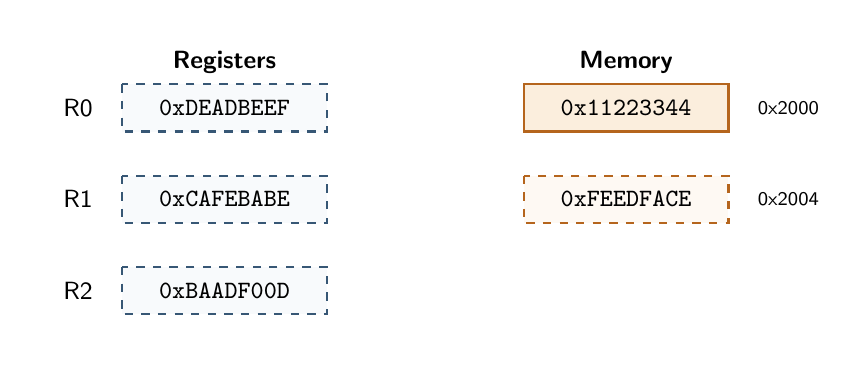
\begin{tikzpicture}[x=10mm, y=8mm]
\path[use as bounding box] (-0.6,1.6) rectangle (9.6,6.9);

\def\rw{2.6}
\def\rh{0.75}
\def\regx{0.6}
\def\memx{5.7}
\def\rowA{6.0}
\def\rowB{4.55}
\def\rowC{3.1}

\node[lbl, font=\sffamily\small\bfseries] at ({\regx+\rw/2},{\rowA+0.35}) {Registers};
\node[lbl, font=\sffamily\small\bfseries] at ({\memx+\rw/2},{\rowA+0.35}) {Memory};

\node[lbl, anchor=east, font=\sffamily\small] at ({\regx-0.25},{\rowA-\rh/2}) {R0};
\draw[extbox] (\regx,\rowA) rectangle ({\regx+\rw},{\rowA-\rh});
\node[font=\ttfamily\small] at ({\regx+\rw/2},{\rowA-\rh/2}) {0xDEADBEEF};

\node[lbl, anchor=east, font=\sffamily\small] at ({\regx-0.25},{\rowB-\rh/2}) {R1};
\draw[extbox] (\regx,\rowB) rectangle ({\regx+\rw},{\rowB-\rh});
\node[font=\ttfamily\small] at ({\regx+\rw/2},{\rowB-\rh/2}) {0xCAFEBABE};

\node[lbl, anchor=east, font=\sffamily\small] at ({\regx-0.25},{\rowC-\rh/2}) {R2};
\draw[extbox] (\regx,\rowC) rectangle ({\regx+\rw},{\rowC-\rh});
\node[font=\ttfamily\small] at ({\regx+\rw/2},{\rowC-\rh/2}) {0xBAADF00D};

\node[lbl, anchor=west, font=\sffamily\scriptsize] at ({\memx+\rw+0.25},{\rowA-\rh/2}) {0x2000};
\draw[memwrite] (\memx,\rowA) rectangle ({\memx+\rw},{\rowA-\rh});
\node[font=\ttfamily\small] at ({\memx+\rw/2},{\rowA-\rh/2}) {0x11223344};

\node[lbl, anchor=west, font=\sffamily\scriptsize] at ({\memx+\rw+0.25},{\rowB-\rh/2}) {0x2004};
\draw[memkeep] (\memx,\rowB) rectangle ({\memx+\rw},{\rowB-\rh});
\node[font=\ttfamily\small] at ({\memx+\rw/2},{\rowB-\rh/2}) {0xFEEDFACE};

\end{tikzpicture}%
}
\end{column}

% ============================== AFTER ===============================
\begin{column}{0.48\textwidth}
\centering{\sffamily\bfseries After}\\[1mm]
\resizebox{\linewidth}{!}{%
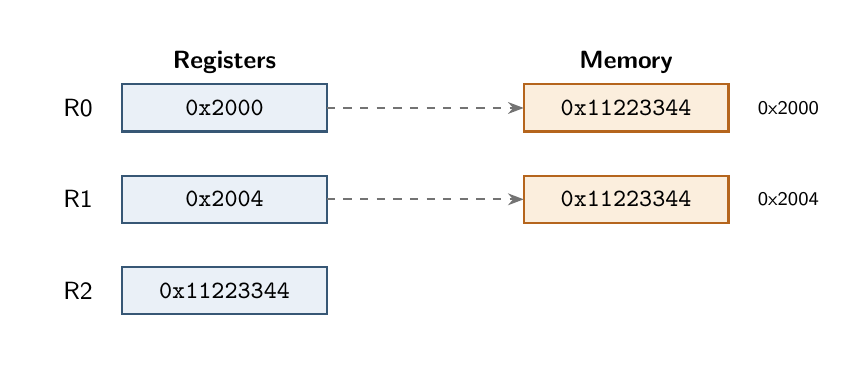
\begin{tikzpicture}[x=10mm, y=8mm]
\path[use as bounding box] (-0.6,1.6) rectangle (9.6,6.9);

\def\rw{2.6}
\def\rh{0.75}
\def\regx{0.6}
\def\memx{5.7}
\def\rowA{6.0}
\def\rowB{4.55}
\def\rowC{3.1}

\node[lbl, font=\sffamily\small\bfseries] at ({\regx+\rw/2},{\rowA+0.35}) {Registers};
\node[lbl, font=\sffamily\small\bfseries] at ({\memx+\rw/2},{\rowA+0.35}) {Memory};

\node[lbl, anchor=east, font=\sffamily\small] at ({\regx-0.25},{\rowA-\rh/2}) {R0};
\draw[loadedbox] (\regx,\rowA) rectangle ({\regx+\rw},{\rowA-\rh});
\node[font=\ttfamily\small] at ({\regx+\rw/2},{\rowA-\rh/2}) {0x2000};

\node[lbl, anchor=east, font=\sffamily\small] at ({\regx-0.25},{\rowB-\rh/2}) {R1};
\draw[loadedbox] (\regx,\rowB) rectangle ({\regx+\rw},{\rowB-\rh});
\node[font=\ttfamily\small] at ({\regx+\rw/2},{\rowB-\rh/2}) {0x2004};

\node[lbl, anchor=east, font=\sffamily\small] at ({\regx-0.25},{\rowC-\rh/2}) {R2};
\draw[loadedbox] (\regx,\rowC) rectangle ({\regx+\rw},{\rowC-\rh});
\node[font=\ttfamily\small] at ({\regx+\rw/2},{\rowC-\rh/2}) {0x11223344};

\node[lbl, anchor=west, font=\sffamily\scriptsize] at ({\memx+\rw+0.25},{\rowA-\rh/2}) {0x2000};
\draw[memwrite] (\memx,\rowA) rectangle ({\memx+\rw},{\rowA-\rh});
\node[font=\ttfamily\small] at ({\memx+\rw/2},{\rowA-\rh/2}) {0x11223344};

\node[lbl, anchor=west, font=\sffamily\scriptsize] at ({\memx+\rw+0.25},{\rowB-\rh/2}) {0x2004};
\draw[memwrite] (\memx,\rowB) rectangle ({\memx+\rw},{\rowB-\rh});
\node[font=\ttfamily\small] at ({\memx+\rw/2},{\rowB-\rh/2}) {0x11223344};

% Address pointers, still true after execution (offset apart so both show)
\draw[-{Stealth[length=2mm]}, dashed, draw=black!55, thick]
    ({\regx+\rw},{\rowA-\rh/2}) -- ({\memx},{\rowA-\rh/2});
\draw[-{Stealth[length=2mm]}, dashed, draw=black!55, thick]
    ({\regx+\rw},{\rowB-\rh/2}) -- ({\memx},{\rowB-\rh/2});

\end{tikzpicture}%
}
\end{column}

\end{columns}

\vspace{2mm}
{\scriptsize\color{black!55} dashed arrow = address used for addressing\par}

\end{frame}

\end{document}
